Since the dot-com era, JavaScript has remained the only client-side language for web browsers. As the web platform gained popularity and its standard APIs expanded, developers became increasingly interested in using faster programming languages on the web. To run these languages on the web, they had to be compiled into a common format, in this case, JavaScript. However, JavaScript, a high-level, dynamically typed, interpreted language, was not intended for this purpose, leading to performance issues.

In 2013, Mozilla engineers introduced a solution called asm.js, which focused on the parts of JavaScript that could be optimized ahead of time. This enabled C/C++ programs to be compiled into the asm.js target format and executed using a JavaScript runtime, achieving faster performance than equivalent JavaScript programs. However, benchmarks revealed that asm.js code ran about 1.5 times slower than the native code written in C++ \cite{zakai_2013_gap}.

As the need for improved web performance persisted, asm.js was replaced by WebAssembly (wasm), introduced in 2015.
“WebAssembly (abbreviated \Gls{WebAssembly}) is a safe, portable, low-level code format designed for efficient execution and compact representation. Its main goal is to enable high performance applications on the Web, but it does not make any Web-specific assumptions or provide Web-specific features, so it can be employed in other environments as well \cite[p.~1]{webassemblycommunitygroup_2023_webassembly}.”
The Wasm standard is developed by W3C Working Group and W3C Community Group. 

\section{Performance}


% \begin{itemize}
%   \item \textbf{Fast}: 
%   \item \textbf{Safe}:
%   \item \textbf{Well-defined}:
%   \item \textbf{Hardware-independent}:
%   \item \textbf{Language Agnosticism}:
%   \item \textbf{Platform-independent}:
% \end{itemize}

\section{Specification}
\label{sec:specification}

phases: \footnote{\url{https://github.com/WebAssembly/meetings/blob/main/process/phases.md}}

\section{Implemented proposals}
\label{sec:implemented-proposals}

\subsection{Multi-Value Return}
In modern programming languages that support tuples, like Kotlin, Rust or Python, developers can effortlessly bundle several values into a single structure for returning from a function. Simple tasks, such as switching a pair of values or sorting an array, become challenging since they must be performed within the linear memory block. Some arithmetic functions, including modular operations and carry bits, can also yield multiple values.

Apart from function return values, another limitation in the WebAssembly MVP is that instruction sequences, such as conditional blocks and loops, cannot consume or return more than one result. It would be equally intriguing to exchange values, perform arithmetic with overflow, or receive a multi-value tuple response in these scenarios as well. Furthermore, compilers are no longer required to jump through hoops when generating multiple stack values for core WebAssembly. This results in smaller generated bytecode and consequently, faster loading times.

\begin{lstlisting}[frame=lines, caption=Simple swap function that evaluates the multi return proposal, captionpos=b, language=JavaScript, showstringspaces=false]
(module
  (func $swap (import "" "swap") (param i32 i32) (result i32 i32))

  (func $mySwapfunc (export "mySwapfunc") (param i32 i32) (result i32 i32)
    (call $swap (local.get 0) (local.get 1))
  )
)
\end{lstlisting}

\subsection{Reference Types}

\subsection{Bulk Memory Operations}


\section{Future proposals}
\label{sec:future-proposals}

\section{Wasm bindgen}
\label{sec:wasm-bindgen}

\section{WebAssembly System Interface (WASI)}
\label{sec:wasi}
While WebAssembly is primarily designed for efficient operation on the web, as previously mentioned, it avoids making web-specific assumptions or integrating web-specific features. The core WebAssembly language remains independent of its surrounding environment and interacts with external elements exclusively through APIs. When operating on the web, it seamlessly utilizes existing web APIs provided by browsers. However, outside the browser environment, there is currently no standardized set of APIs for developing WebAssembly programs. This lack of standardization poses challenges in creating truly portable WebAssembly programs for non-web applications.

The WebAssembly System Interface (abbriveated as WASI) in short is a standard interface for WebAssembly modules to interact with their host environments, such as operating systems, without being tied to any specific host. This allows WebAssembly modules to be executed securely and portably across a wide range of environments. 

% State of WASI
According to Dan Gohman's proposed roadmap, the development of WASI is set to progress through Preview1, Preview2, and Preview3. Presently, the community is actively working on Preview2, ensuring that each milestone contributes to the ultimate goal of a stable and robust WASI 1.0 release. 

\begin{figure}[H]
	\centering
		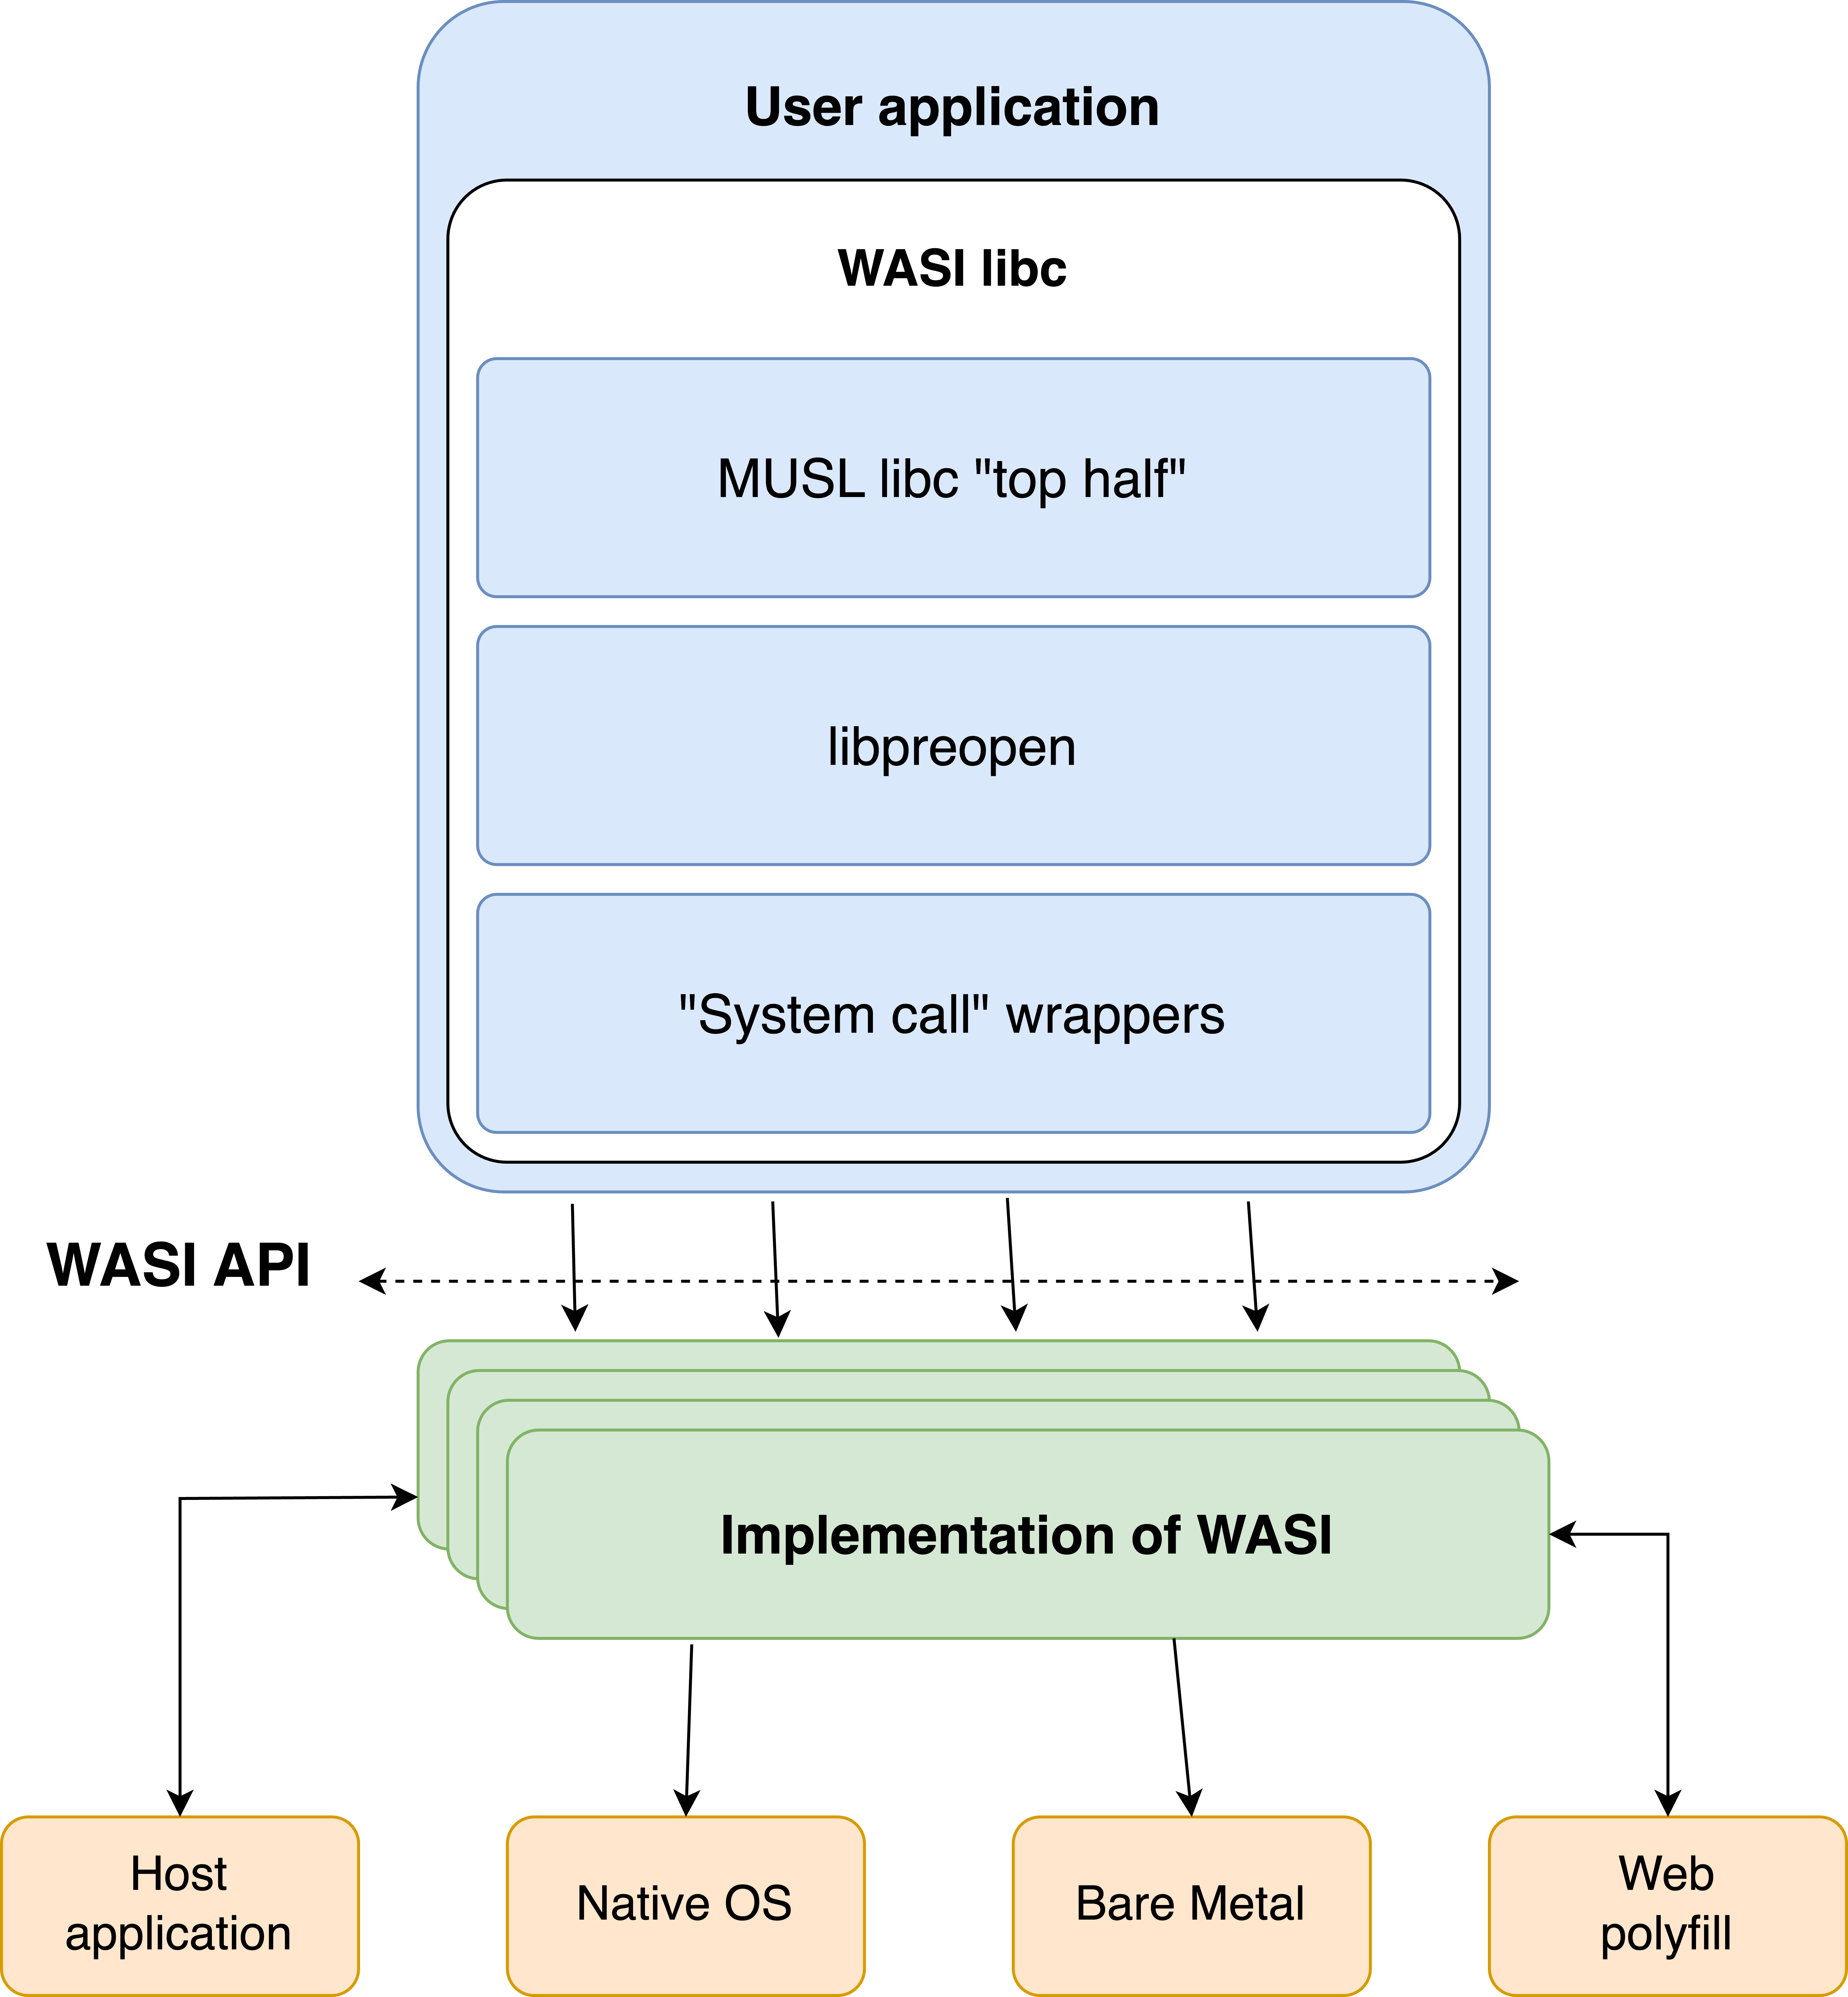
\includegraphics[width=130mm,scale=0.8]{images/wasm/WASI_Architecture.png}
	\caption{WASI Architecture}
	\label{fig:wasi-architecture}
\end{figure}

\subsection{WASI as Emscripten replacement?}
The first toolchain that enabled C, C++, or any other language with \gls{LLVM} support to be compiled into WebAssembly was Emscripten. Essentially, Emscripten can compile almost any portable C or C++ codebase into WebAssembly, encompassing high-performance games requiring graphics rendering, sound playback, and file loading and processing, as well as application frameworks like Qt. Emscripten has been utilized to convert numerous applications like Unreal Engine 4 and the Unity engine, into WebAssembly \cite{emscriptencommunity_2023_emscripten}. 

To achieve this, Emscripten implemented the \gls{POSIX} OS system interface on the web. As a result, developers are able to use the functions available in the C standard library (\gls{libc}). 
Emscripten accomplished this by creating its own implementation of libc, which was divided into two parts. One part was compiled into the WebAssembly module, while the other part was implemented in \gls{JS glue code}. The JS glue would subsequently communicate with the browser, which would in turn communicate with the Kernel and the OS.

\begin{figure}[H]
    \centering
        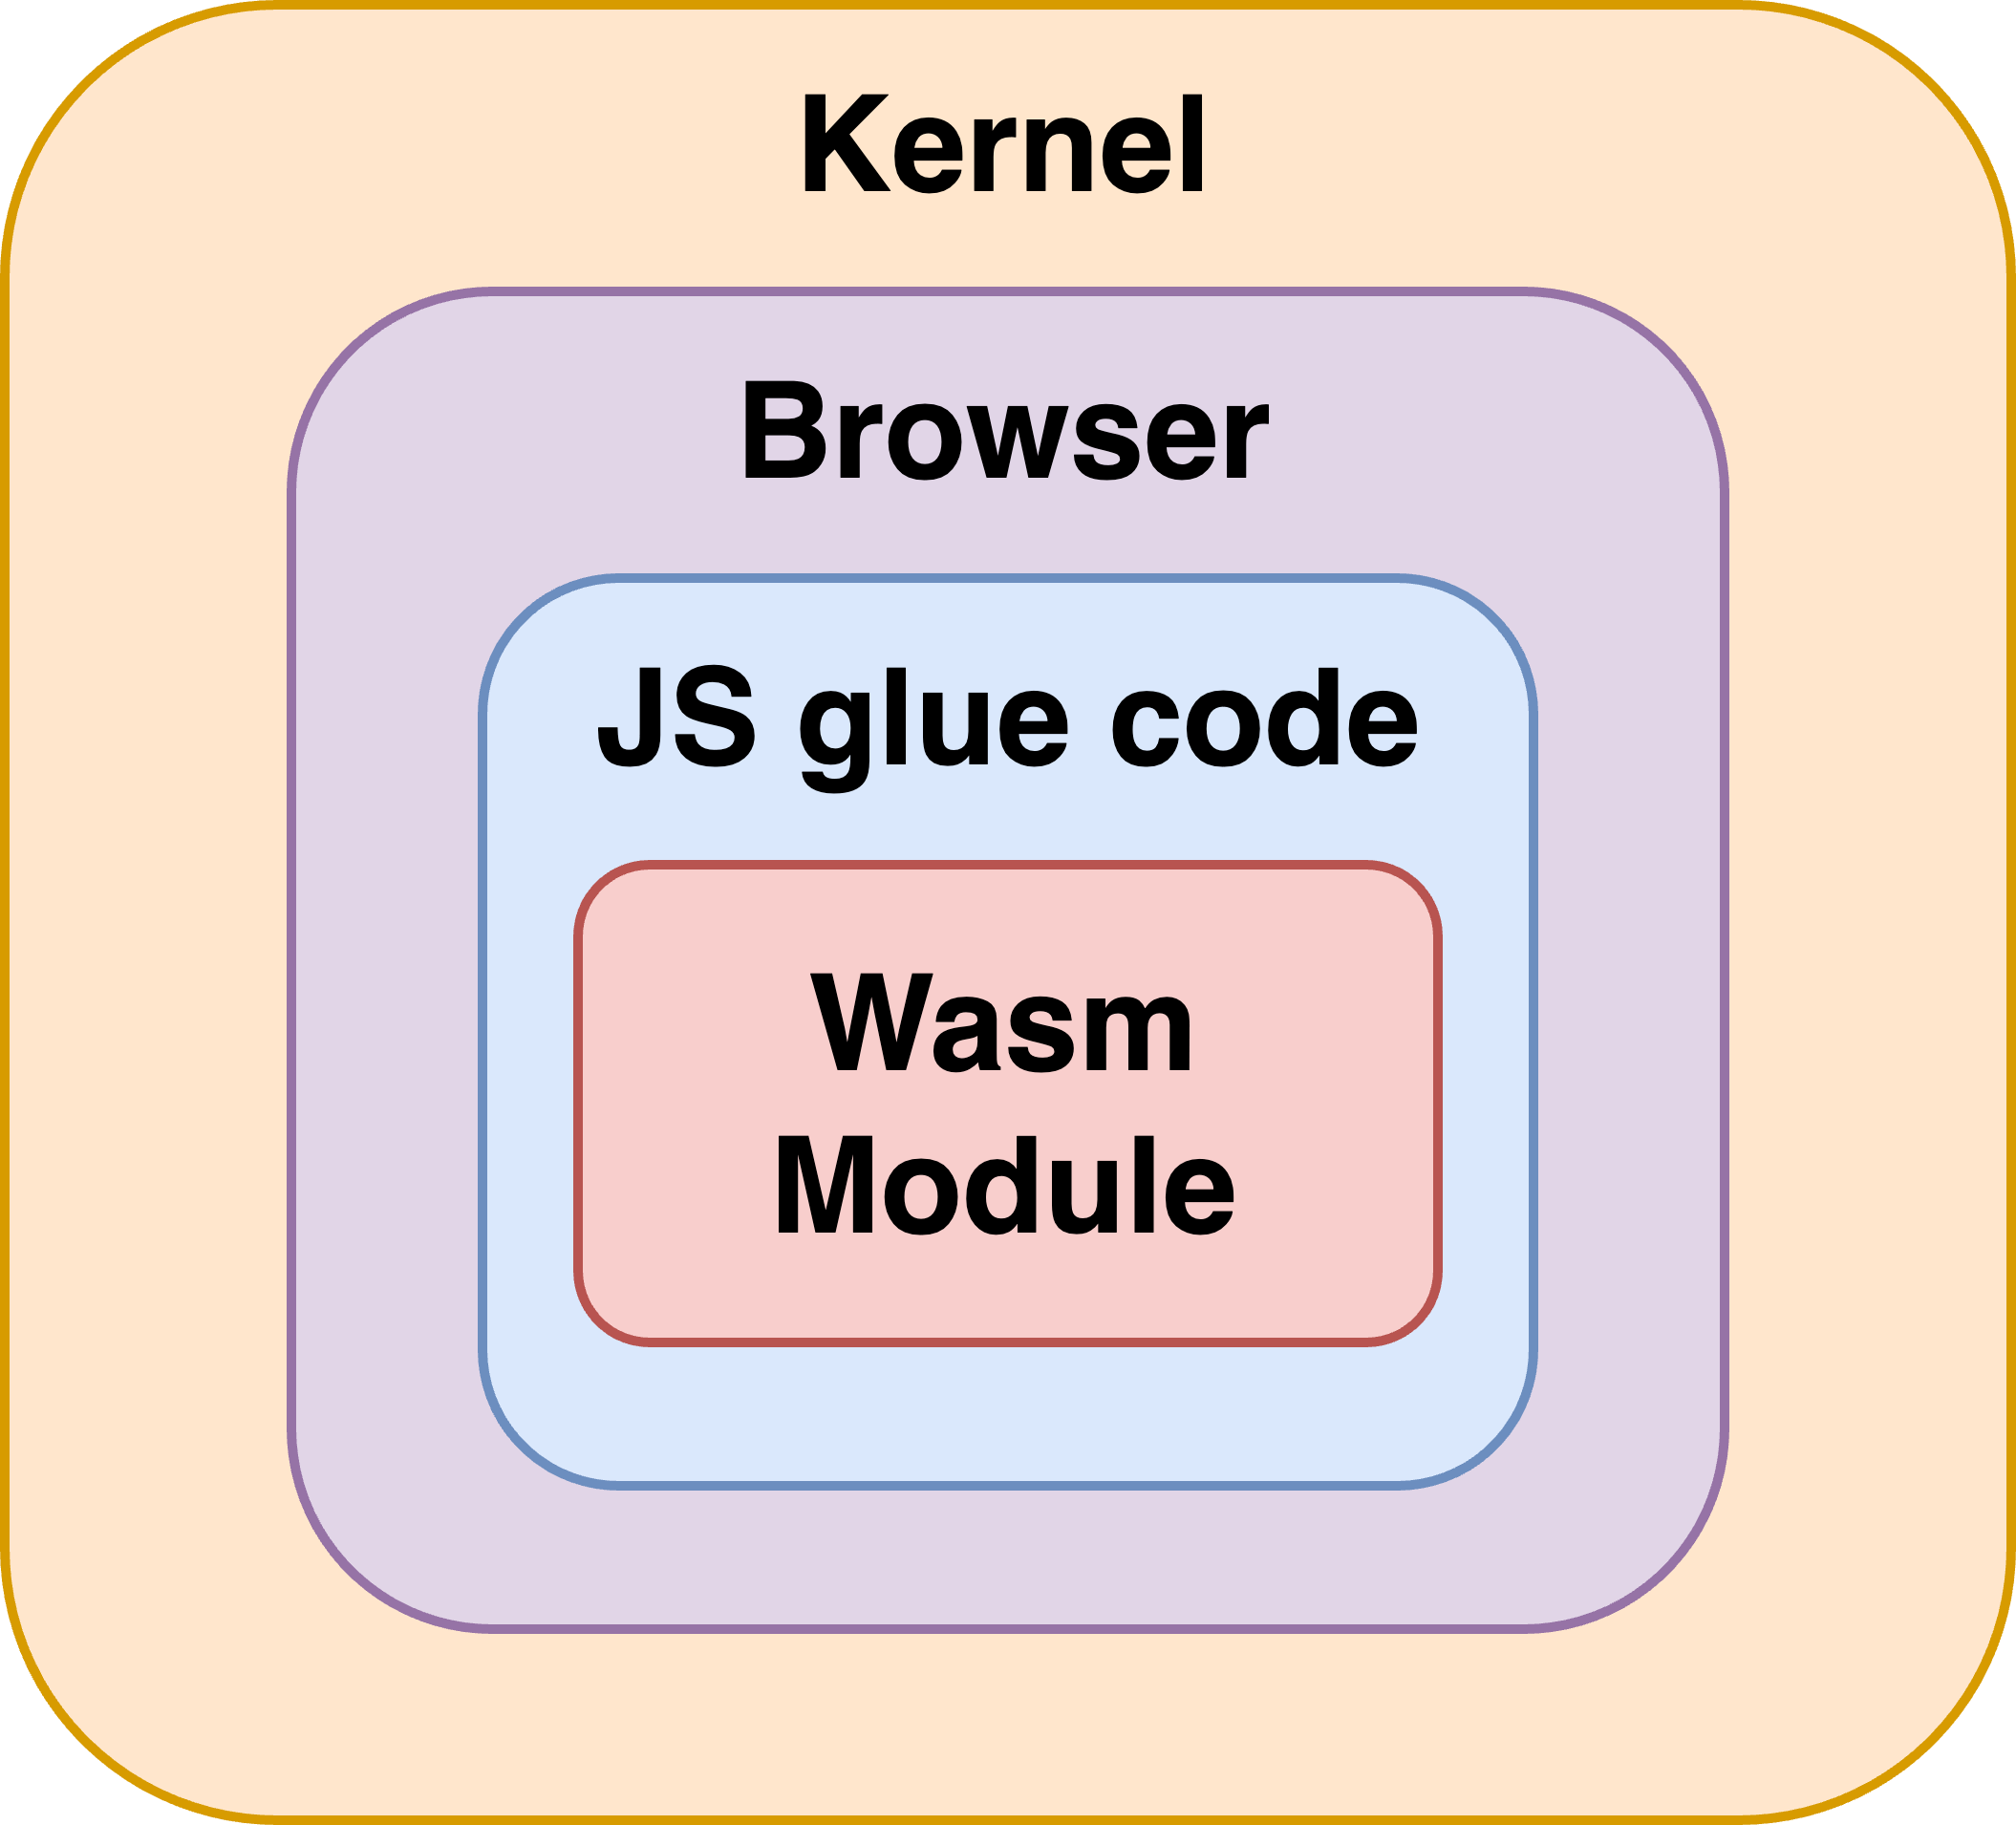
\includegraphics[width=0.6\linewidth]{images/wasm/Emscripten.png}
    \caption{Structure of Emscripten compiled Wasm module}
    \label{fig:emscripten}
\end{figure}

When users began to seek ways of running WebAssembly outside of a browser environment, the first approach was to enable the execution of Emscripten-compiled code on the corresponding environment.
To achieve this, the runtimes had to develop their own implementations of the functions in the JS glue code. However, this presented a challenge as the interface provided by the JS glue code was not intended to be a standard or public-facing interface. It was designed to serve a specific purpose, and creating a portable interface was not part of its intended design. The above figure \ref{fig:emscripten} shows the connection between the browser, the glue code and the Wasm module. 

Emscripten aims to improve the standard by using WASI APIs as extensively as possible in order to minimize unnecessary API differences. As previously stated, Emscripten code accesses Web APIs indirectly via JavaScript on the web. By making the JavaScript API resemble WASI, an unnecessary API difference can be eliminated, allowing the same binary to run on a server as well. In simpler terms, if a Wasm application wants to log information, it must call into JavaScript, following a process similar to this:

\verb|wasm => function musl_writev(...) { ... console.log(...) ... }|

"musl\_writev" represents an implementation of the Linux syscall interface utilized by "musl libc" to write data to a file descriptor, ultimately leading to a call to console.log with the appropriate data. The Wasm module imports and invokes "musl\_writev", thereby defining an ABI between the JavaScript and Wasm components. This ABI is arbitrary, by changing the existing ABI with one that aligns with WASI, the following can be achieved:

\verb|wasm => function __wasi_fd_write(...) { ... console.log(...) ... }|

% X 1. die API zu einem gewissen grad vereinheitlichen kann
% 2. es gibt dinge die emscripten machen kann aber wasi nicht macht
% 3. es macht vielleicht auch sinn eine api für web eine api für server und andere api's für plugins zu haben

%According to \cite{zakai_2019_outside} 

\subsection{WASI Portability}

\begin{figure}[H]
    \centering
        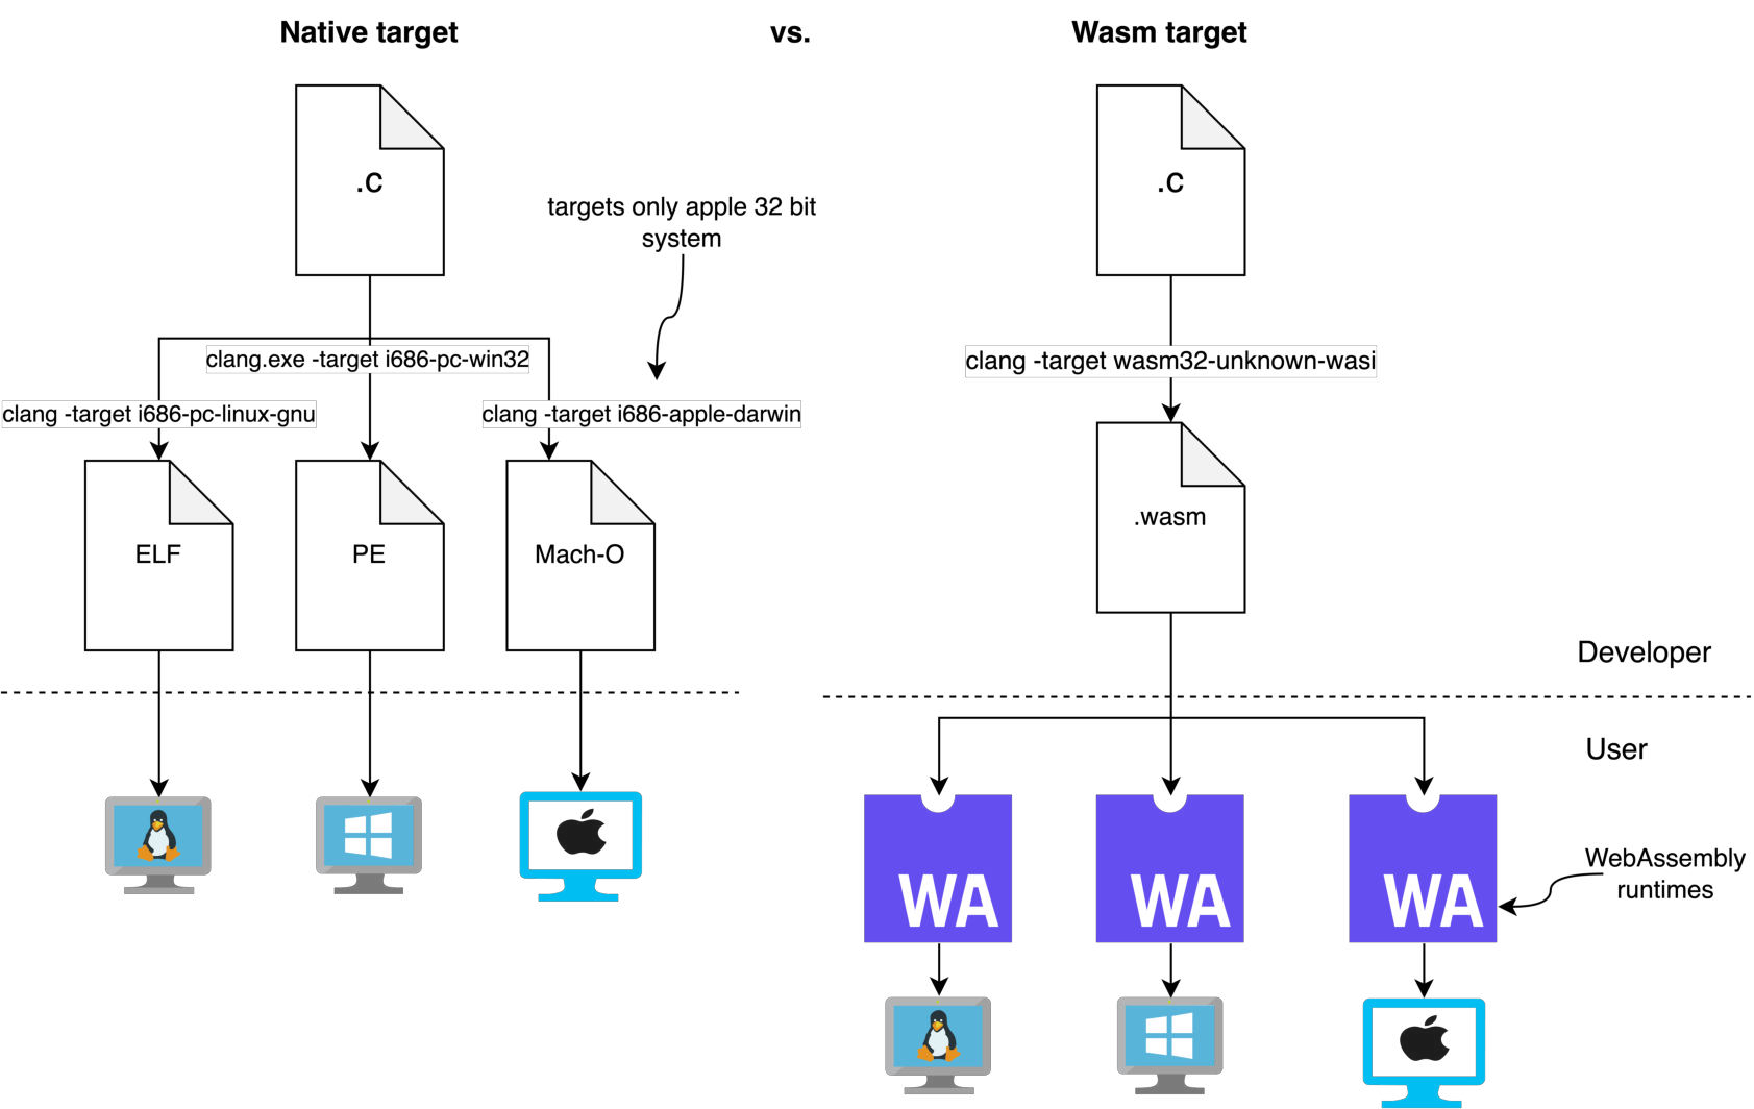
\includegraphics[width=1\linewidth]{images/wasm/WASI_PORTABILITY.pdf}
    \caption{WASI portability model redrawn from \cite{clark_2019_standardising}}
    \label{fig:wasi-portability}
\end{figure}


\subsection{WASI Security Model}
An essential aspect of any system is the security model implemented to ensure the integrity and confidentiality of data and resources. When a code segment requests the operating system (OS) to perform input or output operations, the OS must ascertain whether the action is secure and permissible.

Operating systems generally employ an access control mechanism based on ownership and group associations to manage security. For instance, consider a scenario where a program seeks permission from the OS to access a specific file. Each user possesses a unique set of files they are authorized to access. In Unix systems, for example, the ownership of a file can be assigned to three classes of users: user, group, and others.

Upon initiating the program, it operates on behalf of the respective user. Consequently, if the user has access to the file—either as the owner or as a member of a group with access rights—the program inherits the same privileges. This approach to security helps maintain a robust and reliable system that adheres to the principles of access control and resource protection.

This approach was effective in multi-user systems where administrators controlled software installation, and the primary threat was unauthorized user access. However, in modern single-user systems, the main risk comes from the code that the user runs, which often includes third-party code of unknown trustworthiness. This raises the risk of a supply chain attack, particularly when new maintainers take over open-source libraries, as their unrestricted access could enable them to write code that compromises system security by accessing files or sending them over the network \cite{clark_2019_standardising}.

 % explain supply chain attack

The security aspect of WASI is vital to the universal nature of WebAssembly. The WASI standard was built on a capabilities-based security model, which means the host has to explicitly permit capabilities such as file system access and establishing network sockets. As a result, a WASI module cannot run arbitrary code with direct access to memory.

% todo reference to a filesystem example wasmtime and wasmer

